%%
%% 第四章
%% 2014.6.27
\chapter{重建算法系统设计及仿真结果}



\section{系统设计}

本文综合使用上述两章提到的图像重建算法和相似图像搜索技术,在文献\cite{Yue:2013gl}系统的基础上进行了完善,设计了针对大数据集的图像重建系统。系统分为离线训练和在线搜索两部分组成,如图\ref{fig:system}所示。

\begin{figure}
\centering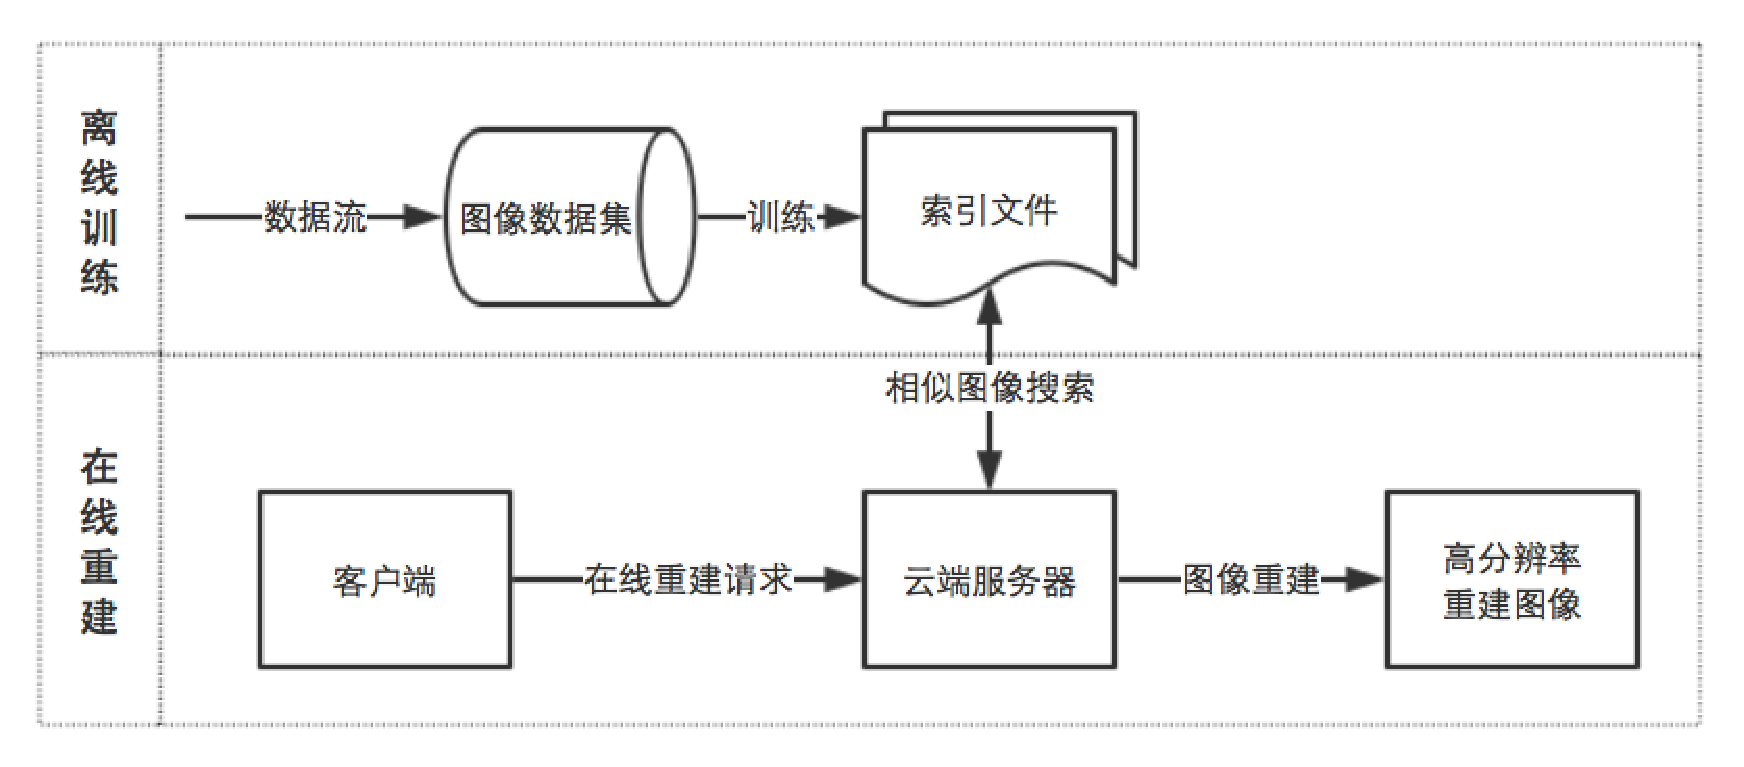
\includegraphics[width=15cm]{imgs/ch4/system}
\caption{服务器在线重建流程图}
\label{fig:system}
\end{figure}

\subsection{离线训练系统}
服务器离线训练系统主要是针对大图像数据集构建索引,分为这样几个步骤:
\begin{enumerate}
\item 提取数据库中每一幅图像的局部特征,本文使用的是SIFT特征。SIFT特征需要进行关键点检测、关键点过滤、二次曲线拟合,计算梯度等一些列操作,运算量大相对耗时。因为每一幅图像是独立的,这一步可以使用并行算法,将图像分布式的存储在多台机器上,分别进行局部特征提取。
\item 对全体特征进行抽样,选择全体特征描述子的一个子集。
\item 对描述子子集使用上文提到的近似K均值聚类AKM,生成视觉词码表。视觉词码表将作为后续所有局部特征的量化标准,一旦对视觉词码表更新,所有局部特征对应的分类也需要更新。
\item 根据视觉词码表,对局部特征全集进行分类计算,计算最近邻的方式与AKM中寻找最近邻类目的计算方式一致,都是采用随机K-D树森林的方式进行高效查询。每一幅图像得到一个视觉词的集合。
\item 并行处理每一幅图像,针对每一幅图像的视觉词打包编码生成视觉词组表示方式。
\item 对视觉词组构建倒排索引,生成倒排索引表。倒排索引表的
\end{enumerate}


\subsection{在线重建系统}
客户端-云端在线重建系统如图\ref{fig:serverOnline}所示。

\begin{figure}
\centering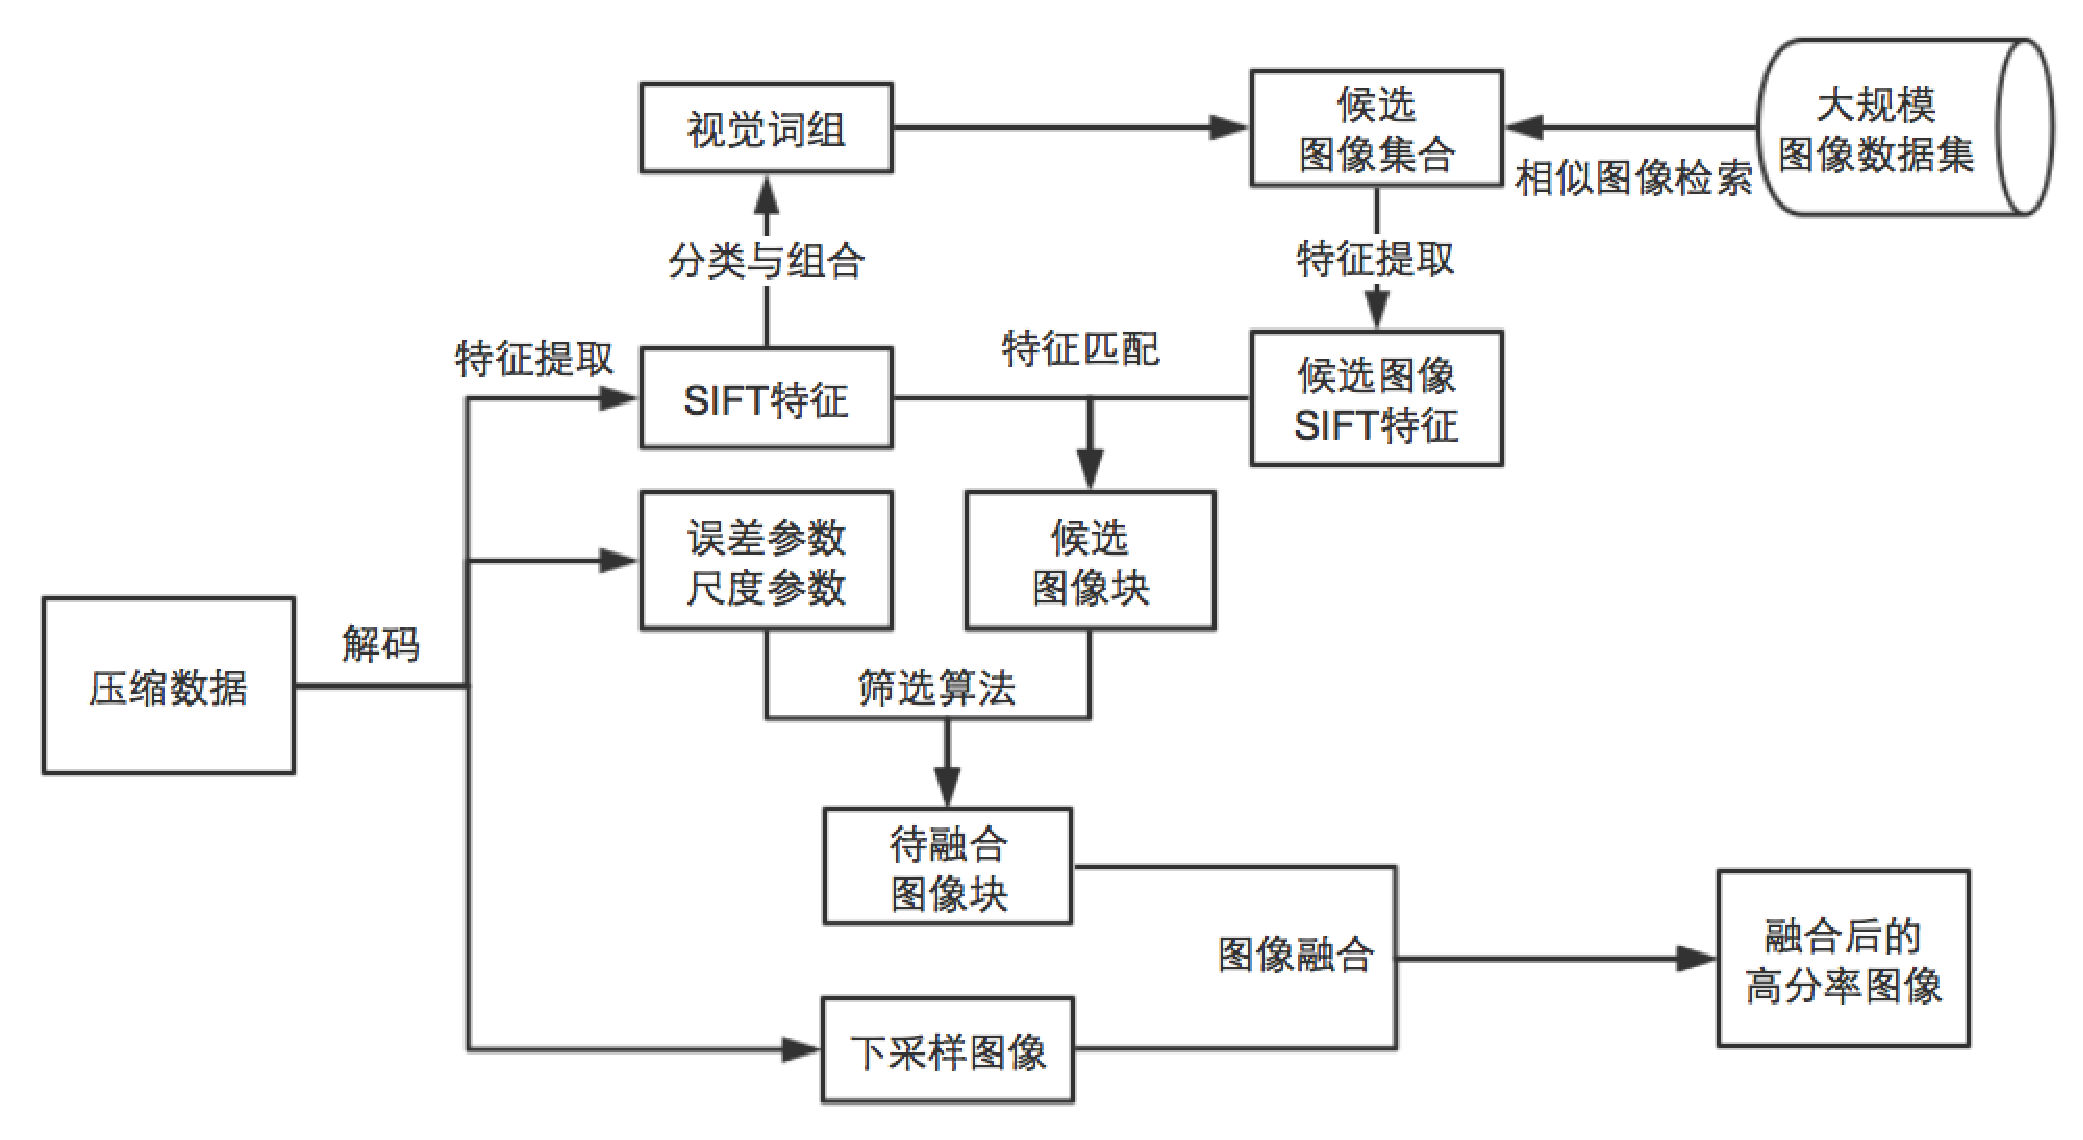
\includegraphics[width=15cm]{imgs/ch4/serverOnline}
\caption{服务器在线重建流程图}
\label{fig:serverOnline}
\end{figure}

从客户端传输来的压缩编码的数据包含了三部分信息,分别是(1)下采样图像,是1:256比例进行采样的图像,服务器端利用插值法进行上采样,恢复成原始大小得到\(I_u\);(2)SIFT关键点,传送给服务器的特征仅仅包含关键点的位置、尺度、方向等信息,不包含128维的描述子,服务器需要根据上述信息在图像\(I_u\)上重新计算特征描述,做进一步的匹配工作(3)控制信息,包括误差控制参数中的基准误差和图像块的尺度控制等,尺度控制数值与客户端提取SIFT特征计算时有关,在客户端提取时一幅图像包含各个尺度上大量的SIFT算子,通常我们需要设定一定的尺度门限,只传输门限以上的特征,这个门限可以通过SIFT算子的数量不同动态的设定。设定的门限对服务器端的候选图想块过滤起到一定的影响,所以我们将尺度门限作为控制参数传递给服务器,近一步指导候选图像块的筛选。

经过上述计算,我们解码得到三类数据,运用上文提到的视觉词组编码方式计算视觉词组,对原始图像进行分块后,在大规模图像集上利用倒排索引进行快速的相似图像搜索,得到了候选图像集合。对候选图像进行SIFT提取后与原始图像的SIFT进行匹配得到候选图像块,使用控制参数对候选图像块进行筛选得到待融合图像块,最后在下采样图像的指导下使用经典的泊松图像编辑\cite{Perez:2003ul}对图像块进行由大到小的融合,最终得到一幅高分辨率的图像。

\section{实验结果}
本文在Matlab和Python环境下仿真了上述的图像重建系统,使用VL-FEAT图像处理函数库
\cite{vl_feat}进行SIFT特征提取,使用其中相似K聚类(Approximately K-Means)进行视觉词的量化分类。数据集使用的是INRIA Holiday数据集\cite{INRIA},包含了500组共1491个人旅游照片,图像集中平均每幅图像的分辨率在五百万像素以上。选择了其中三十张图像进行重建,其它图像作为大图像数据集进行训练。其中三幅图像的实验结果如图\ref{fig:result}所示。其中第一列是原始图像,第二列是采用较大数值作为误差阈值时的重建结果,第三列是采用较小数值作为误差阈值时的重建结果,第四列是采用自适应阈值法时的重建结果。

\begin{figure}
\centering
\includegraphics[width=15cm]{rec_result}
\caption{图像重建结果}
\label{fig:result}
\end{figure}

可以看到第一幅图像在阈值较大、误差条件宽松时对图像的重建效果好;第二幅像在阈值较小、误差条件苛刻时还原效果好;第三幅图像在误差阈值较大时出现错误匹配,而在较小时又有大面积的区域匹配不到任何候选图像块。采用自动阈值的方式进行图像重建,三幅图像的重建的效果比较理想。实验结果表明,采用自动阈值进行候选图想块筛选的方式虽然不能保证每一幅图像都获得最佳的重建结果,但在大部分情况下它能保证还原的图像有着较佳的主观视觉效果。

\ifx\usechapbib\empty
\nocite{BSTcontrol}
\bibliographystyle{buptgraduatethesis}
\bibliography{bare_thesis}
\fi
